\section{Analyzing Families of DSLs with \textsc{PuzzleMetrics}}
\label{sec:metrics}

\subsection{Visualizing the family's shape}

The first step in the evaluation of potential reuse in a family of DSLs is to understand the types of relationships existing among the family members. We need to identify if there domains are either independent (in which case the set of DSLs can not be considered as a family), overlap or are hierarchically organized. To do so, the first capability we offer in our framework is the construction of a Venn diagram that shows the matches at both the abstract syntax and the semantics. 

Figure \ref{fig:shape}. shows the corresponding family's shape for the case of our motivating scenario. In that figure we can see that the family is an overlapping family in terms of the abstract syntax. In the case of the semantics the results are quite interesting. Note that depending on the type of comparison operator we have different results. When the comparison operator is the naming, we have the same overlapping shape that in the case of the abstract syntax. However, when the operators become more restrictive the overlapping region is reduced. 

\begin{figure}
\centering
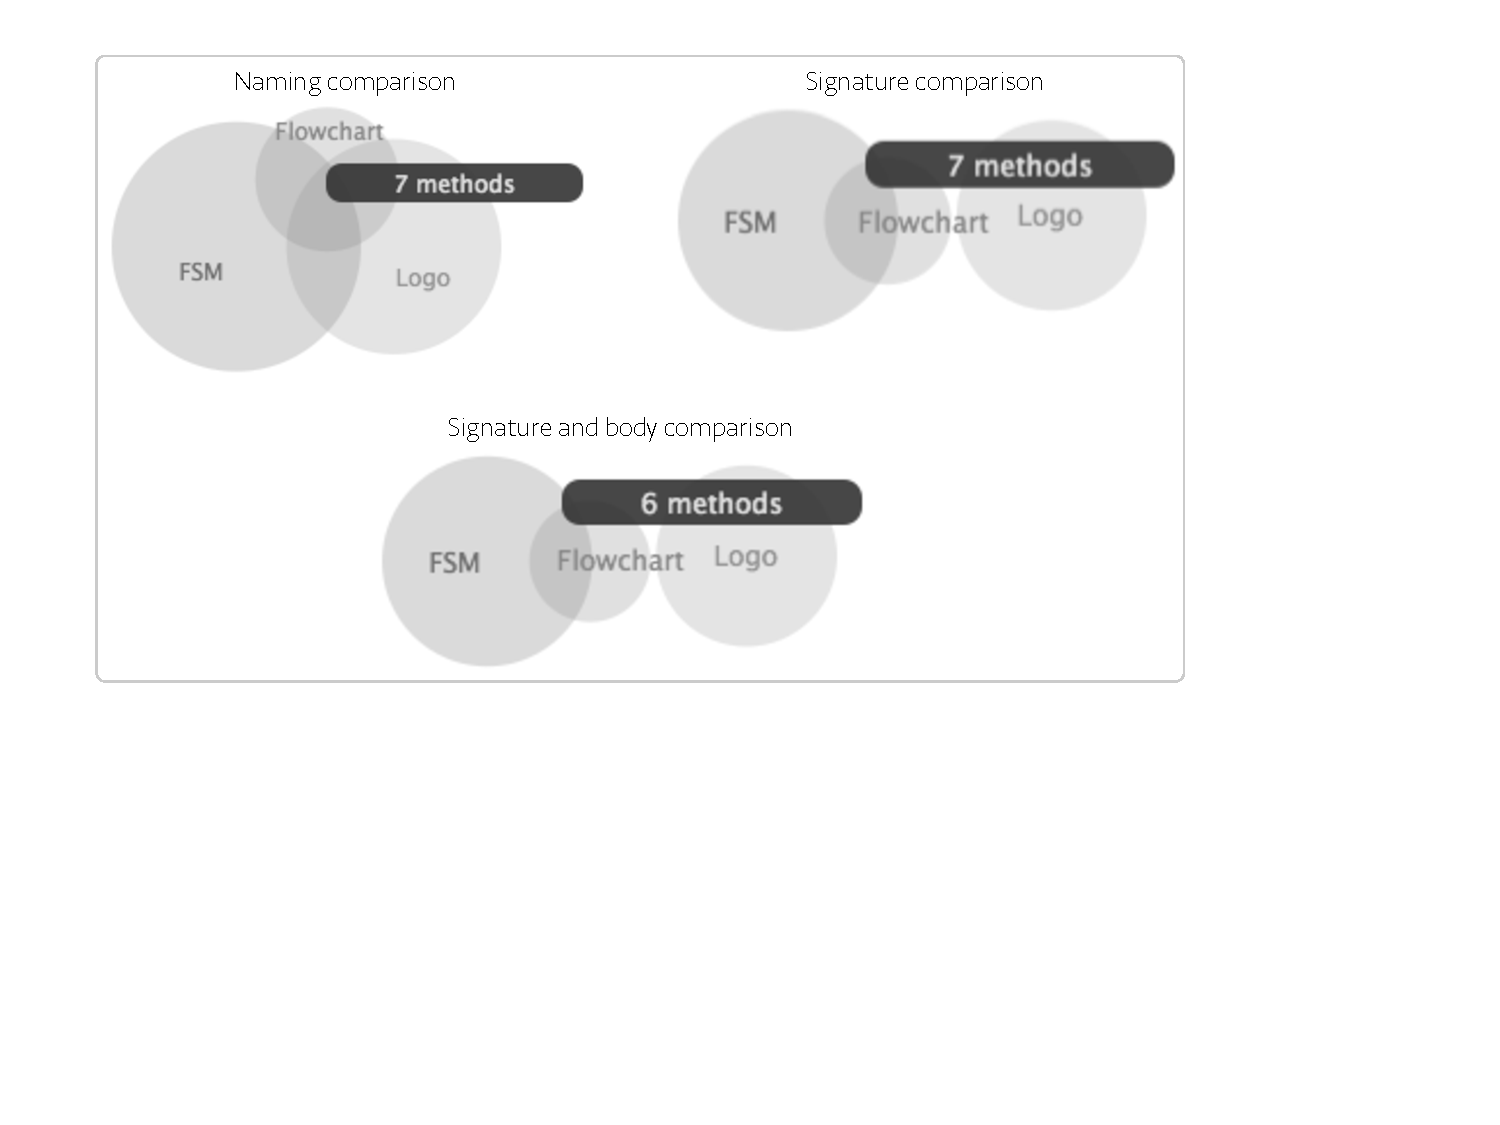
\includegraphics[width=1\linewidth]{images/shape-fig.pdf}
\caption{Visualizing family's shape according to the selected comparison operator}
\label{fig:shape}
\end{figure}

\subsection{Evaluating the family's potential reuse}

The second part of our analysis corresponds to a quantitative evaluation of potential reuse. To do so, we include the reuse metrics presented in X and we adapt them for the case of families of DSLs. In this section we present these metrics in terms of the formulas we used to compute them based on the basic definitions presented in section X. Besides, we show the output that our tool provides for our motivating scenario. 

\begin{itemize}
\item \textbf{Size of Commonality (SoC):} This metric shows the size of the core with respect to the rest of the family. It is calculated as the percentage of constructs/methods that are included in the core with respect to the union of the constructs/methods of all the DSLs of the family.

\hspace{3mm} The usefulness of this metric is associated to  the fact that the existence of a core is quite important to determine if a family of DSLs is candidate for producing a language product line. Although the fact that a family does not contains a core is not necessarily discards the family as a candidate for building a software product line, there are certain consencious about the importance of a core. In fact, there are certain approaches where the first restriction is that the core exists. Moreover, in the case of language product lines there are authors that propose approaches that can only be used if the core exists. 

\hspace{3mm} On the other hand, the larger the core the smaller the variability. So the amount of required decomposition is reduced and the variability model is simpler. So, one may think that a family where the core is big is a family where the variability is easier to manage. 

\vspace{2mm}
\item \textbf{Product-Related Reusability ($PRR_i$):}
This metric shows the percentage of reuse of each DSL with respect the core. Concretely, it shows for each product the amount of constructs/methods that are included in the core.

\hspace{3mm} This metric is important because we can detect the product more related to the core. This identification will be helpful at the moment of defining that core. 

\vspace{2mm}
\item \textbf{Individualization Ratio ($IR_i$):}
This metric shows the percentage of reuse of each DSL with respect the rest of the family. Concretely, it shows for each product the amount of constructs/methods that are included in at least another DSL that is member of the family.

\hspace{3mm} This metric is important because it allows the identification of the most isolated product as well as the most integrated to the family.

\vspace{2mm}
\item \textbf{Pairwise Relationship Ratio ($PWRR_{(i,j)}$):} 
This metric shows the percentage of reuse of each DSL with respect the each of the other DSLs that are members of the family. Concretely, it shows, for each product, the amount of constructs/methods that are included each of the other members of the family.
\end{itemize}

\subsection{Visualizing family's variability}

After being evaluated the potential reuse of the family under study we go deeper in the details and we show the variability. In the case of the functional variability, we show a graph that shows us the constructs of all the family, the DSLs they belong to and the relationships they have with other constructs. This is useful since it is a first income to the reverse engineering process. In fact, as state in Y, the first step towards the reverse-engineering process is to break down a language. Besides, the modularization problem can be seen as a graph partitioning problem. Our analysis provides this graph. 

In the case of the semantical variability we show the different versions of the DSAs available for each construct.

